This appendix describes how the photovoltaic series is prepared, forecast and scored for \autoref{sec:results}. It covers three pieces of work: an inspection of the record day by day, a single forecast examined in detail, and a benchmark over many windows spread across the year. All three are descriptive, and the series is the application domain of the study and is used for high-level insight only.

\subsection{The record}

The series is the module power of the SolarTech Lab plant\autocite{levaPhotovoltaicPowerWeather2020}, recorded once per minute over the whole of 2017, $525{,}601$ timestamps in total. Only $198{,}730$ of them, $37.8\%$, carry a valid reading. Power is absent outside daylight by construction, because the plant produces nothing and the logger records nothing; during the day readings are also lost whenever the logger misses a minute. Twenty readings above $1$\,kW, with a maximum near $60$\,kW, are physically impossible for this module and are treated as missing rather than as data.

Each day is inspected by locating its longest run of consecutive valid readings, which is the longest stretch that could be handed to a model without any filling. The longest run in the whole year is $880$ minutes, on 5 July, and only $64$ of the $365$ days reach the $544$ consecutive readings used by the synthetic windows. \autoref{fig:solarOverlay} superimposes four days of different character: clear summer days follow a smooth arc, a winter day produces less power over a shorter interval, and a cloudy day departs from the arc in rapid drops and peaks that last a few minutes each. Those departures come from the weather and not from the plant, so they are part of what a forecaster is asked to predict and cannot learn from the context.

\begin{figure}[!htbp]
    \centering
    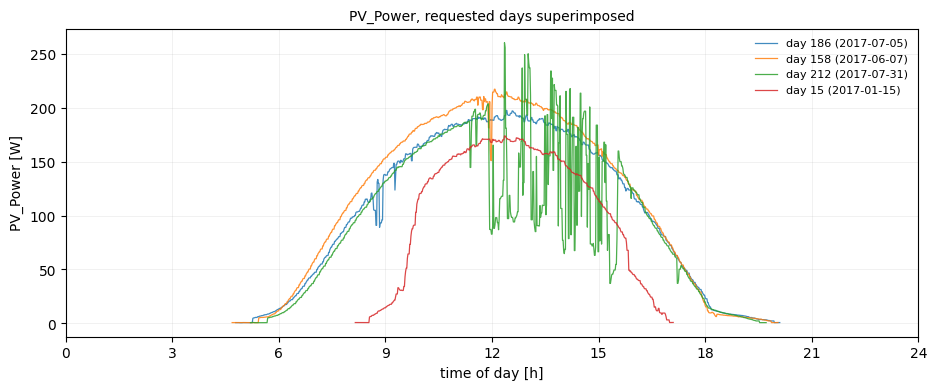
\includegraphics[width=0.9\textwidth]{figures/SOLAR_days_overlay.png}
\caption{Module power on four recorded days, superimposed by time of day: two clear summer days (5 July and 7 June), a summer day with passing clouds (31 July) and a winter day (15 January). Gaps in a curve are minutes without a valid reading.}
    \label{fig:solarOverlay}
\end{figure}

\subsection{From a record with gaps to a model input}

A context is the $2048$ minutes that precede the moment the forecast is issued, taken as they fall in the record, so it always crosses at least one night and usually reaches into the previous day. Because the model cannot be given an absent value, every missing minute of the context is resolved by one of three rules. A minute with the sun below the horizon, computed from the site coordinates and the date, is set to zero, since that is the power the plant actually produces then. A daytime gap of at most $15$ minutes is bridged by a straight line between the valid readings on either side of it. Any remaining daytime gap is also set to zero, and is the only filling that may differ from what the plant did. In the benchmark the bridging uses only readings that precede the forecast time, so no information from the horizon enters the context.

The horizon is treated differently, because it is what the forecast is scored against. A horizon minute is kept if it was measured, or if it falls at night, where its value is known to be zero. A missing daytime minute is excluded from the score rather than filled, since its true value is not known.

\subsection{Reading minutes in cycles per patch}

The tokeniser sees a sequence of samples and has no notion of seconds, so the series is given to the model as it is, without resampling. A component whose period is $T$ samples completes $P/T$ cycles in a patch and $S/T$ in a stride, whatever the sampling rate, and the candidate condition of \autoref{sec:tokenisation}, a whole number of cycles per patch or per stride, reads the same on this series as on the synthetic signals. At one sample per minute and $P=S=16$, the first candidate sites are periods of $16$, $8$ and $16/3$ minutes. Variations of that speed exist in the record only as the short weather transients described above; the dominant content of a window is the daily cycle, whose period is some hundred times longer.

\subsection{One forecast in detail}

A single forecast is first examined in detail, issued at 13:00 on 5 July 2017, the day with the longest valid run, and repeated for the published checkpoint and for every retrained geometry on the same context. It complements the winter forecast of \autoref{sec:results} with a summer day of a different kind: the context starts at 02:52 on the previous day, $1377$ of its $2048$ minutes are measured, $634$ night-time minutes are set to zero, $37$ minutes of short daylight gaps are bridged, and all $64$ horizon minutes are measured.

\begin{figure}[!htbp]
    \centering
    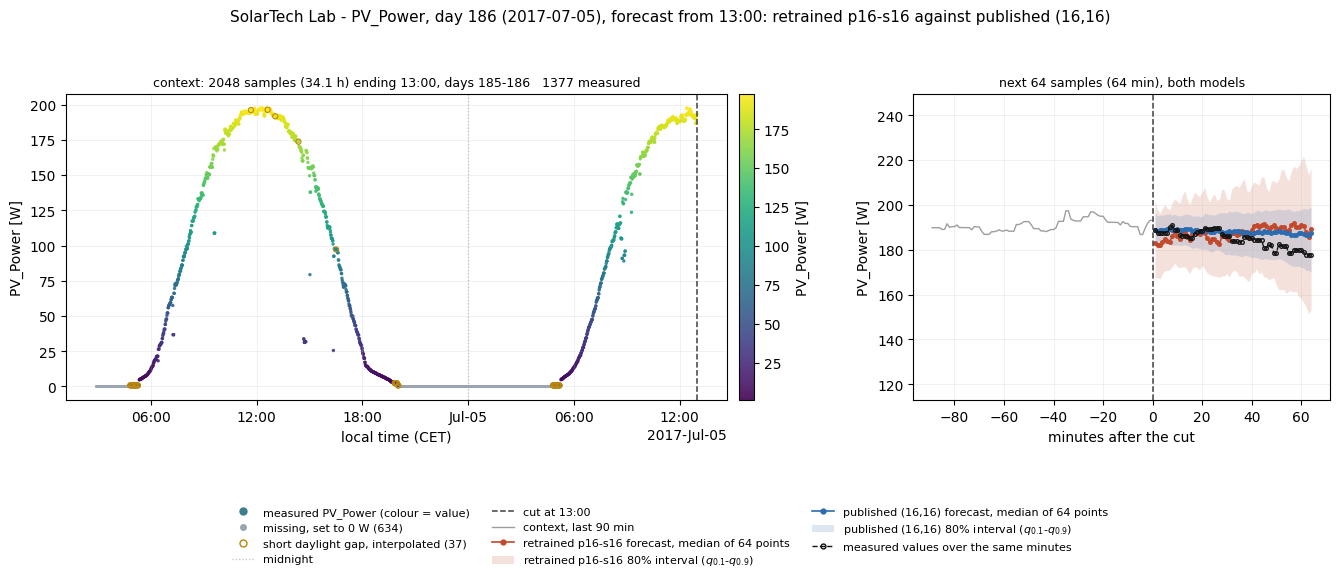
\includegraphics[width=\textwidth]{figures/SOLAR_day186_1300_p16-s16_both.png}
\caption{Forecast issued at 13:00 on 5 July 2017 by the retrained $P=S=16$ geometry and by the published checkpoint. Left, the full context with its measured, zero-filled and interpolated minutes marked; right, the last $90$ minutes of context and the $64$ forecast minutes, with each model's median and $80\%$ interval against the measured values.}
    \label{fig:solar186both}
\end{figure}

\autoref{fig:solar186both} and \autoref{fig:solar186err} show the reference geometry against the published checkpoint. Both continue the midday level near $188$\,W while the measured power starts to decline after about half an hour, and both intervals contain all $64$ measured minutes. The error is small in either case, $5.3$\,W for the retrained model and $3.8$\,W for the published one, and it grows along the horizon as the two medians stay flat above a falling measurement.

\begin{figure}[!htbp]
    \centering
    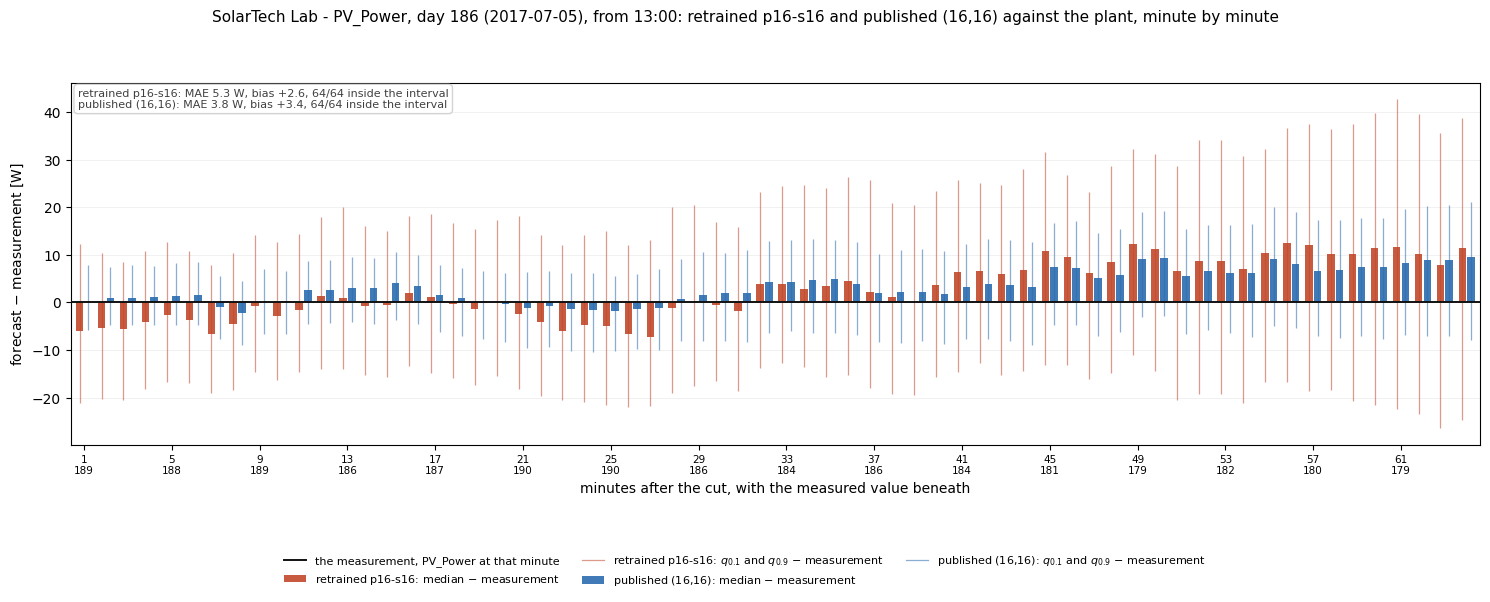
\includegraphics[width=\textwidth]{figures/SOLAR_day186_1300_p16-s16_error.png}
\caption{The same forecast as \autoref{fig:solar186both}, drawn as the difference between forecast and measurement minute by minute: bars for the medians, thin lines for the $10\%$ and $90\%$ quantiles, with the measured value printed beneath each labelled minute.}
    \label{fig:solar186err}
\end{figure}

Across the fifteen geometries the same cut gives errors between $5.3$ and $15.9$\,W. \autoref{fig:solar186patch} groups their medians by patch size, and the forecasts spread over about $40$\,W at $P=24$ and $P=32$, some rising and some falling, while the measurement moves by ten watts, and within a patch size the order of the curves does not follow the stride. One cut on one day cannot separate the geometry from the particular window, which is why the benchmark below repeats the comparison over many windows.

\begin{figure}[!htbp]
    \centering
    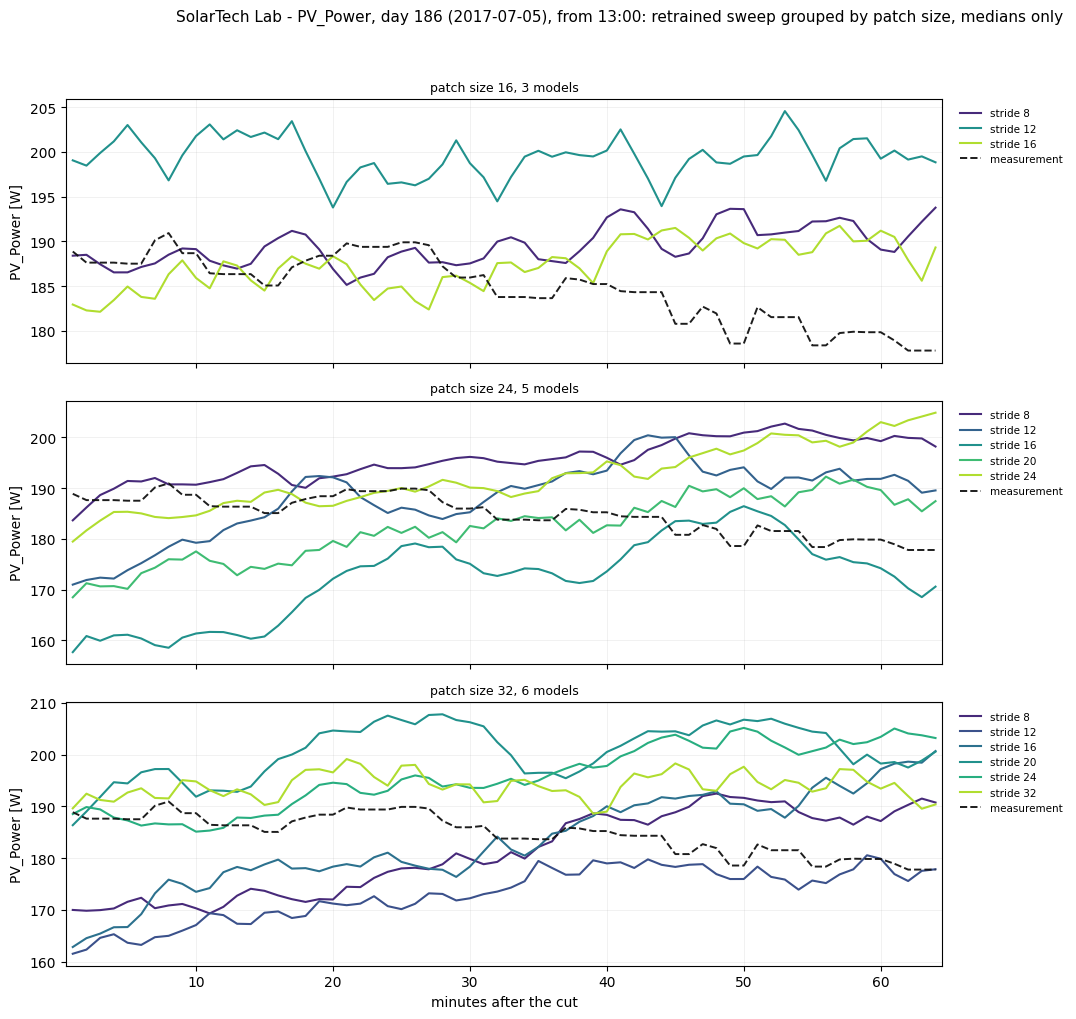
\includegraphics[width=0.8\textwidth]{figures/SOLAR_day186_1300_bypatch.png}
\caption{Median forecasts of the retrained geometries for the cut of \autoref{fig:solar186both}, one panel per patch size and one colour per stride, against the measured values (dashed). Intervals are omitted so that the curves remain readable.}
    \label{fig:solar186patch}
\end{figure}

\subsection{The benchmark over the year}

The benchmark draws $150$ windows of $2048+64$ minutes each, chosen at random over the whole year under the constraint that no two windows share a minute, from a fixed seed so that the selection can be reproduced. Every model forecasts exactly the same windows from exactly the same contexts, and every model is scored on the same minutes. Each scored minute is assigned to one of three regimes, night, the transitions around sunrise and sunset, and day, so that the near-zero night-time error does not dilute the daytime one.

The point forecast is the median of the nine quantiles each model returns. For each model the mean absolute error, the mean error or bias, the variance of the error and the root mean square error are computed over all scored minutes, and the weighted quantile loss is computed over all nine quantiles to judge the forecast distribution rather than its median alone. Each model is also compared with two references, the published checkpoint and the retrained $P=S=16$, through the paired difference in mean absolute error. Its interval comes from a bootstrap that resamples whole weeks, $51$ of them, $2000$ times, so that windows falling in the same week are not treated as independent. An interval that contains zero means the two models cannot be told apart on this series; it does not mean that they are equal.

\autoref{tab:solarPrediction} in \autoref{sec:results} reports the errors and the comparison with the retrained baseline, and \autoref{tab:solarVsOfficial} reports the quantile loss and the comparison with the published checkpoint. Every retrained geometry is worse than the published model, by between $1.9$ and $7.6$\,W apart from the outlying p32-s20, and the quantile loss orders the models almost exactly as the mean absolute error does, while \autoref{fig:solarSummary} draws the three error measures side by side.

\begin{table}[!htbp]
    \centering
    \small
    \renewcommand{\arraystretch}{1.1}
    \begin{tabular}{@{}ccccc@{}}
        \toprule
        & & & \multicolumn{2}{c}{\textbf{$\Delta$MAE vs published}} \\
        \cmidrule(l){4-5}
        \textbf{$P$} & \textbf{$S$} & \textbf{WQL} & \textbf{Estimate} & \textbf{Interval} \\
        \midrule
        $16$ & $16^{\dagger}$ & $0.152$ & --- & --- \\
        \midrule
        $8$ & $8$ & $0.210$ & $+3.16$ & $[1.97,\,4.37]$ \\
        \midrule
        $16$ & $8$ & $0.191$ & $+1.91$ & $[1.08,\,2.79]$ \\
        $16$ & $12$ & $0.291$ & $+6.65$ & $[4.96,\,8.43]$ \\
        $16$ & $16$ & $0.200$ & $+2.52$ & $[1.40,\,3.63]$ \\
        \midrule
        $24$ & $8$ & $0.247$ & $+5.08$ & $[3.63,\,6.59]$ \\
        $24$ & $12$ & $0.206$ & $+3.16$ & $[2.18,\,4.23]$ \\
        $24$ & $16$ & $0.271$ & $+6.44$ & $[4.55,\,8.43]$ \\
        $24$ & $20$ & $0.300$ & $+7.59$ & $[5.72,\,9.50]$ \\
        $24$ & $24$ & $0.212$ & $+3.29$ & $[1.85,\,4.65]$ \\
        \midrule
        $32$ & $8$ & $0.275$ & $+6.37$ & $[4.89,\,7.79]$ \\
        $32$ & $12$ & $0.242$ & $+4.72$ & $[3.23,\,6.21]$ \\
        $32$ & $16$ & $0.251$ & $+5.39$ & $[3.93,\,6.90]$ \\
        $32$ & $20$ & $0.638$ & $+24.59$ & $[19.10,\,30.00]$ \\
        $32$ & $24$ & $0.248$ & $+5.29$ & $[3.79,\,6.90]$ \\
        $32$ & $32$ & $0.198$ & $+2.61$ & $[1.71,\,3.53]$ \\
        \bottomrule
    \end{tabular}
\caption{The probabilistic side of the benchmark and the comparison with the published checkpoint. WQL is the weighted quantile loss averaged over the nine forecast quantiles, lower being better; the last two columns give the paired difference in MAE, in watts, from the published checkpoint (row $\dagger$), with the same week-resampling bootstrap interval as \autoref{tab:solarPrediction}.}
    \label{tab:solarVsOfficial}
\end{table}


\begin{figure}[!htbp]
    \centering
    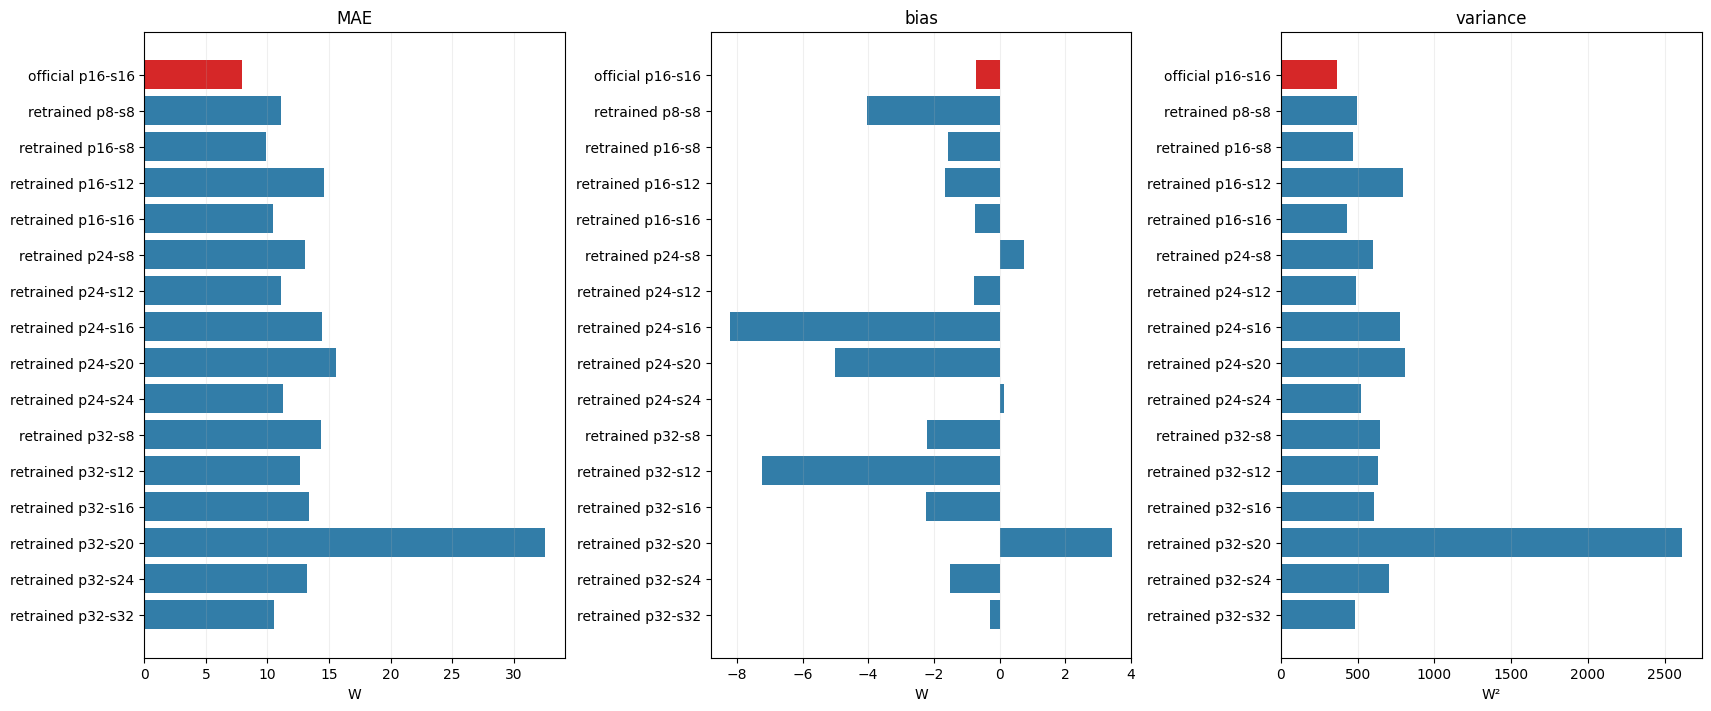
\includegraphics[width=\textwidth]{figures/SOLAR_benchmark_summary.png}
\caption{Mean absolute error, bias and error variance of the median forecast over the $150$ windows, for the published checkpoint (red) and the fifteen retrained geometries (blue).}
    \label{fig:solarSummary}
\end{figure}

\subsection{The dominant frequency of the context}

To place each window in the units of \autoref{sec:tokenisation}, the strongest non-constant component of its context is located on the Hann-windowed spectrum of the $2048$ context minutes, after the mean is removed. Only the context is used, so nothing about the horizon enters this coordinate. Across the $150$ windows that component falls on one of the three lowest frequencies the context can resolve, which are periods of about $34$, $17$ and $11$ hours: $108$ windows on the first, $40$ on the second and $2$ on the third. In cycles per patch this is at most $0.05$ for any geometry, so the dominant content of every window is the daily envelope and none lies near a candidate site. \autoref{fig:solarFreq} reports the error of each model grouped by that component. The error tends to fall as the dominant period shortens, but the groups are of very unequal size and differ in season and weather, so the figure describes the sample rather than a property of the geometry.

\begin{figure}[!htbp]
    \centering
    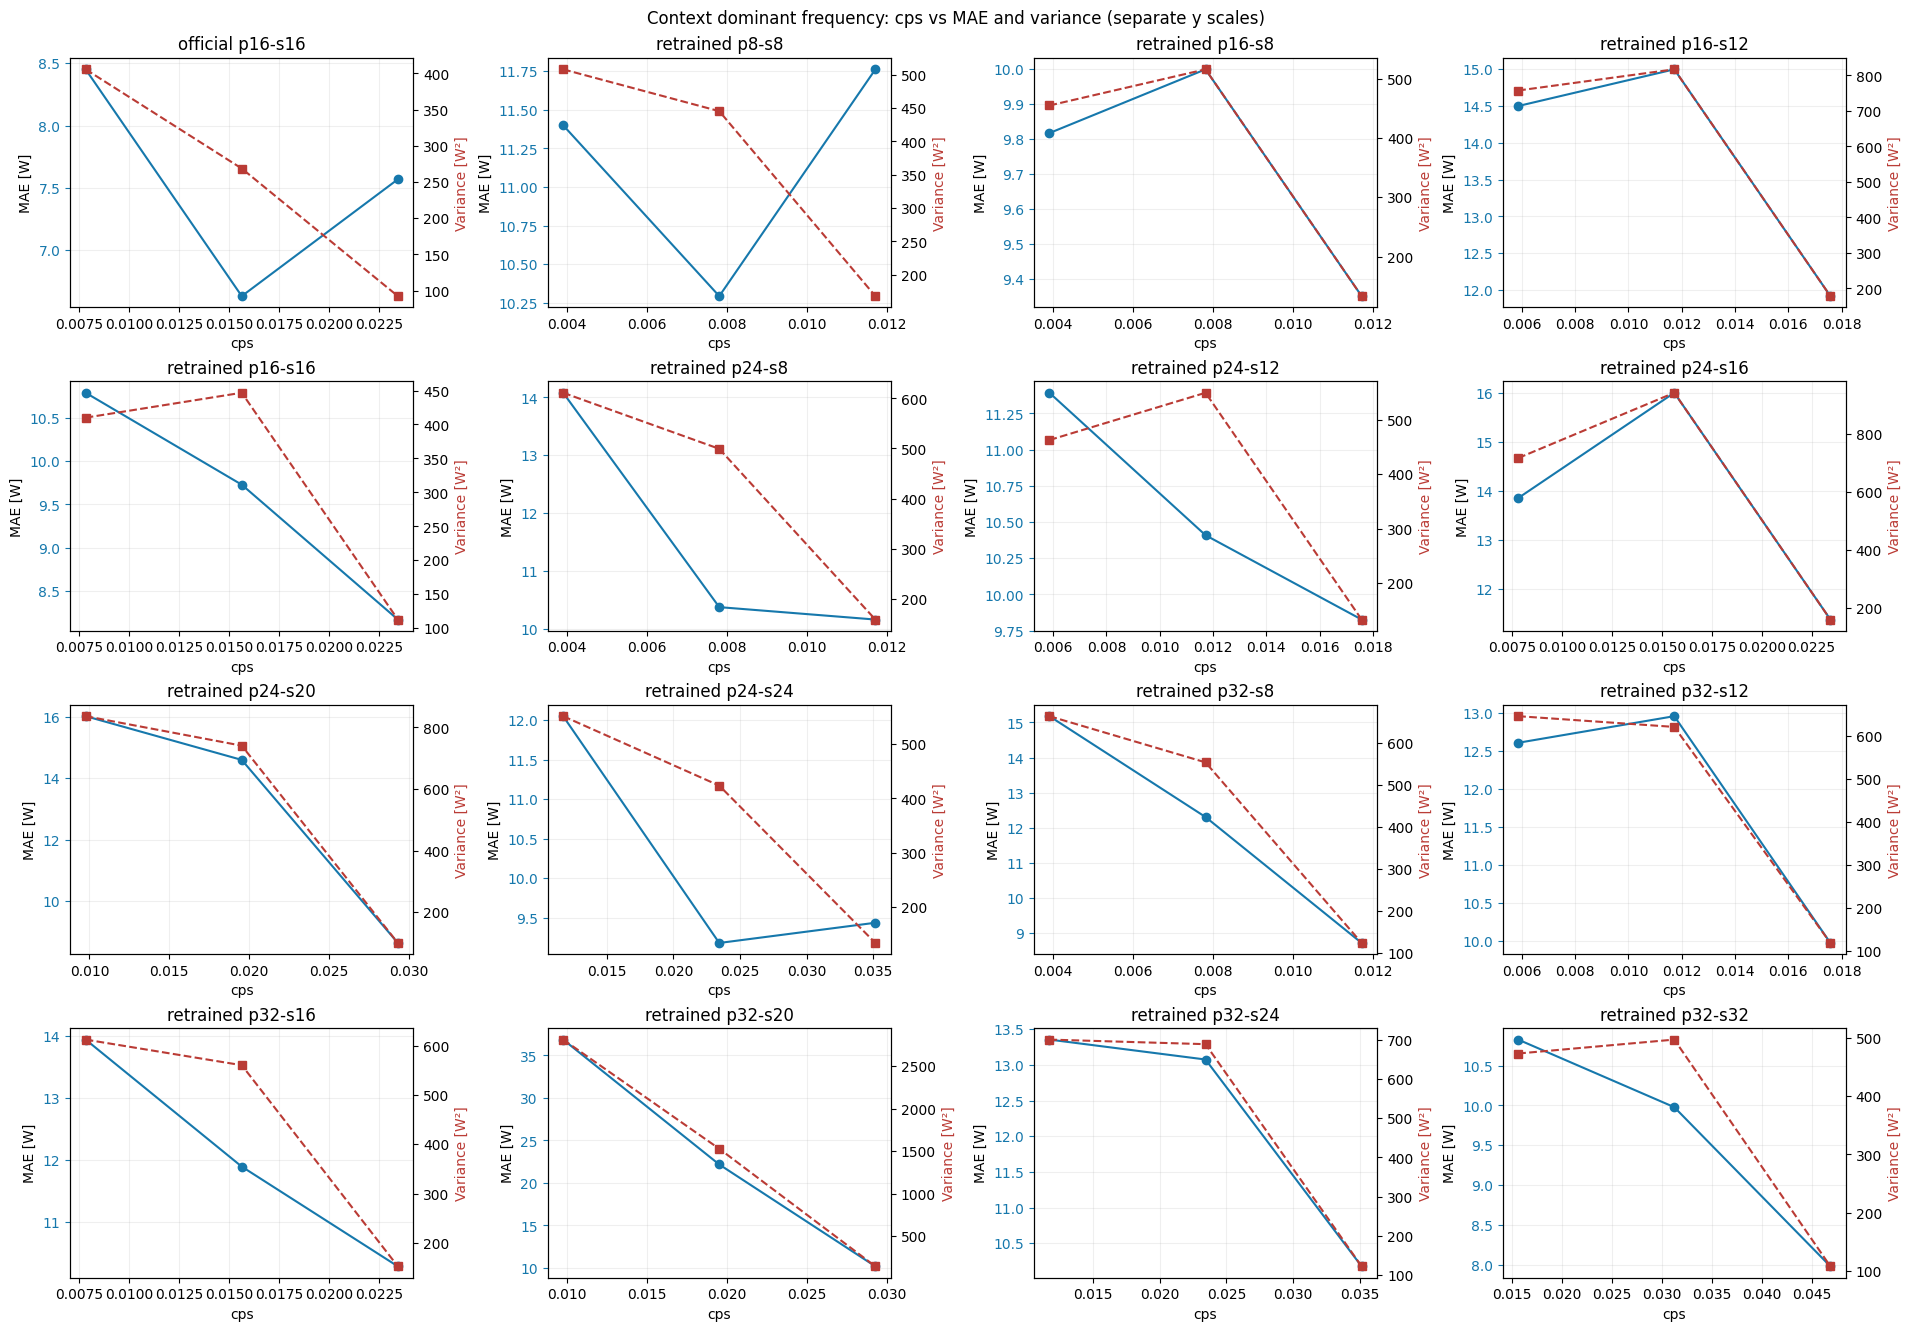
\includegraphics[width=\textwidth]{figures/SOLAR_benchmark_frequency_cps.png}
\caption{Mean absolute error (solid, left axis) and error variance (dashed, right axis) of each model, grouped by the dominant frequency of the context, expressed in cycles per stride of that model's geometry. The three points of each panel hold $108$, $40$ and $2$ windows respectively.}
    \label{fig:solarFreq}
\end{figure}

\subsection{Limits}

The benchmark covers one plant and one year, and the published checkpoint was trained with a different data mixture and procedure, possibly including series of this kind, whereas the retrained models follow the original Chronos T5 recipe, so its advantage cannot be attributed to geometry; only the comparison among the retrained models isolates the geometry, and on this series it shows no geometry better than the $P=S=16$ baseline. The zero-filling of night-time minutes is exact, but the zero-filling of long daytime gaps in the context is an assumption. Finally, the p32-s20 checkpoint produces power at night and errs more than twice as much as any other model; that behaviour belongs to the checkpoint and should be verified before it is read as an effect of the geometry.
